\documentclass[xcolor=svgnames,titlepage,english,presentation]{beamer}
\usetheme{HUB}

\makeatletter
\let\HUB@realinsertinstitute\insertinstitute
\makeatother

\setbeamercovered{invisible}
\usepackage[noborder,colbullets]{beamerMACSYdefs}
\usepackage[normalem]{ulem}
% -----------------------------------------------------------------------------
% -- packages
\usepackage{framed}
\usepackage{amsmath}
\usepackage{amssymb}
\usepackage{amsthm}
\usepackage{graphicx}
\usepackage{colortbl}
\usepackage{bbding}
\usepackage{booktabs}
\usepackage{adjustbox}
\usefonttheme[onlymath]{serif}
\usetikzlibrary{patterns,positioning}
\usetikzlibrary{decorations.pathreplacing}
\usetikzlibrary{positioning}
\usepackage[absolute,overlay]{textpos}


\HUBfaculty{HU Berlin}

\graphicspath{{./images/}}

\setbeamertemplate{title page}[mydefault]

% -----------------------------------------------------------------------------

\title{Memory-aware Adaptive Scheduling of Scientific Workflows On Heterogeneous Architectures}
\subtitle{}

\author[S. Kulagina]{\underline{Svetlana Kulagina$^1$}, Anne Benoit$^2$ and Henning Meyerhenke$^{1,3}$}

%\institute{
%   \begin{minipage}{\linewidth}
%        \centering
%%        $^1$: Department of Computer Science, Humboldt-Universit\"at zu Berlin, Germany\\
%       $^2$: LIP, ENS Lyon, France\\
%        $^3$: Institute of Informatics, Humboldt-Universit\"at zu Berlin, Germany
%   \end{minipage}
%}

%\parbox{\linewidth}{
%    $^1$: Department of Computer Science, Humboldt-Universit\"at zu Berlin, Germany  \\
%%    $^2$: Department of Computer Science, Humboldt-Universit\"at zu Berlin, Germany \\
%    $^3$: Department of Computer Science, Humboldt-Universit\"at zu Berlin, Germany
%}


%\TitleImage[width=0.3\textwidth]{diagrams/cropped-1024px-FONDA_LogoLogo.jpg}



\begin{document}

\setlength\textheight{7cm} %required for correct vertical alignment, if [t] is not used as documentclass parameter

%%%%%%%%%%%%%%%%%%%%%%%%%%%%%%%%%%%%%%%%%%%
\makeatletter
\begin{frame}[plain]
   % \setbeamertemplate{frametitle}{}
    \setbeamercolor{background canvas}{bg=white}

    % ——— recreate HUB frame & logos ———
    \begin{tikzpicture}[remember picture,overlay]
        \fill[white] (current page.north west) rectangle (current page.south east);
        \draw[HUBrframe,line width=\HUB@RFramewd]
        (current page.north west) rectangle (current page.south east);

        % Top-right HUB logo
        \node[anchor=north east,inner sep=8pt] at (current page.north east)
            {\pgfimage[width=25\K@mm]{\HUB@logo}};
        % Bottom-right MACSy logo
        \node[anchor=south east,inner sep=8pt] at (current page.south east)
            {\pgfimage[width=25\K@mm]{\MACSY@logo}};
    \end{tikzpicture}

    % ——— content ———
    \vfill
    \begin{center}
    {\usebeamerfont{title}\usebeamercolor[fg]{title}\color{HUBblue}\LARGE\bfseries
    Memory-aware Adaptive Scheduling of Scientific Workflows\\
    On Heterogeneous Architectures\par}
                \vskip1.5em
            {\usebeamerfont{author}\usebeamercolor[fg]{author}\small
        \underline{Svetlana Kulagina$^1$}, Anne Benoit$^2$ and Henning Meyerhenke$^{1,3}$\par}
        \vskip1.5em

        % Custom institute box
        \setlength{\fboxsep}{0.8em}
        \colorlet{myBG}{HUBblue!15}
        \colorlet{myFG}{HUBblue!80}
        \fcolorbox{myFG}{myBG}{%
            \parbox{0.75\textwidth}{\centering
                $^1$ Humboldt‑Universität zu Berlin, Germany\\
                $^2$ LIP, ENS Lyon and IUF, France\\
                $^3$ Karlsruhe Institute of Technology (KIT), Germany
            }%
        }
        \vskip2em

        % Title image
        \usebox{\HUB@titimg}
    \end{center}
    \vfill

\end{frame}
\makeatother

%%%%%%%%%%%%%%%%%%%%%%%%%%%%%%%%%%%%%%%%%%%%%

\begin{frame}[t]
    \frametitle{Motivation}

    \begin{itemize}
        \item Large applications represented as DAG-shaped workflows
        \item Heterogeneous execution environment with limited memories
         \begin{itemize}
                  \item Exceed memory = expensive or even fatal
        \end{itemize}
        \item Execute the workflow fast
    \end{itemize}   

\begin{columns}
    \column{0.59\textwidth}
    \begin{figure}
            \centering
            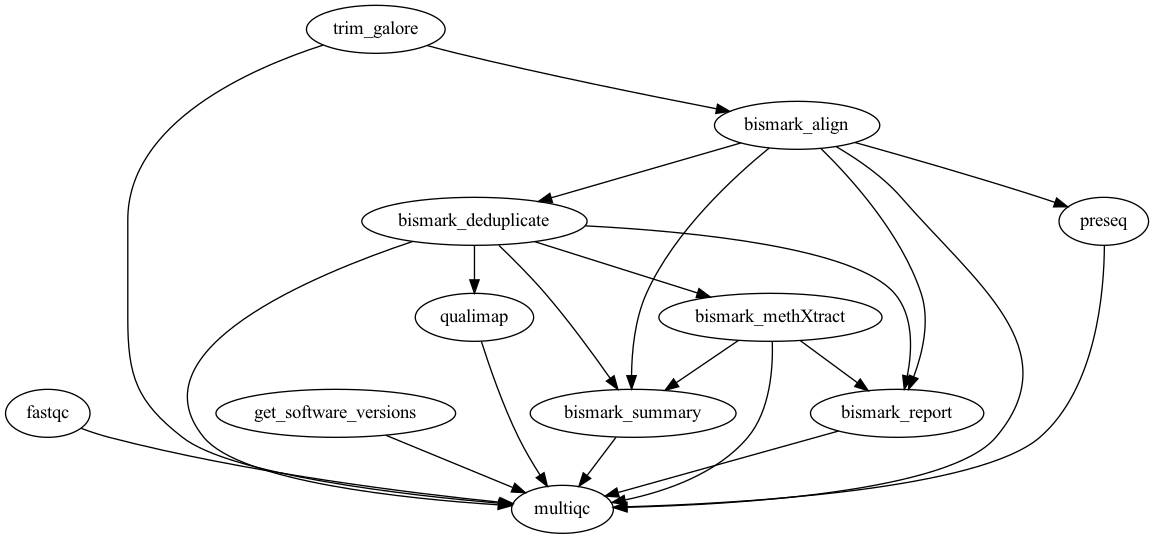
\includegraphics[scale=0.25]{diagrams/images/methylseq-sparse.png}
            
            %\caption{Caption }
        \end{figure}
    \column{0.39\textwidth}
    \only<1>{
     \begin{figure}
            \centering
            \includegraphics[scale=0.3]{diagrams/images/CCGrid-muffin.png}
            
            %\caption{Caption }
        \end{figure}
    }
    \only<2>{
     \begin{figure}
            \centering
            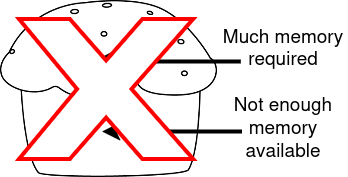
\includegraphics[scale=0.3]{diagrams/images/CCgrid-muffin-no.png}
            
            %\caption{Caption }
        \end{figure}
    }
   
\end{columns}
   


\end{frame}

%%%%%%%%%%%%%%%%%%%%%%%%%%%%%%%%%%%%%%%%%%%%%

\begin{frame}[t]
    \frametitle{Contributions}

    3 variants of a HEFT-based scheduler: HEFTM-\textbf{BL}, HEFTM-\textbf{BLC}, and HEFTM-\textbf{MM}

    ~~~~~~~~~~~~~~~~~

    
    \begin{itemize}
        \item Respects processor memory sizes
        \begin{itemize}
            \item HEFTM-\textbf{BL} and HEFTM-\textbf{BLC} produce valid makespans that are only $10$-$35\%$ worse than invalid HEFT makespans
            \item HEFTM-\textbf{MM} able to schedule all workflows even under extreme memory constraint
        \end{itemize}
        
        \item + adaptive strategy for scenario with uncertainty          

        \begin{itemize}
            \item Adapting the schedule leads to $>20\%$ makespan improvement even on smallest workflows
        \end{itemize}
    
    \end{itemize}

    
    

\end{frame}


%%%%%%%%%%%%%%%%%%%%%%%%%%%%%%%%%%%%%%%%%%%%%%%%%%%
\begin{frame}[t]
    \frametitle{Model: Workflow}
   

    ~~~~~
   
 

      \begin{columns}
      
        \column{0.4\textwidth}
         \begin{itemize}
             \item Tasks have \textcolor{orange}{memory} and \textcolor{magenta}{workload} weights
             \item Edges have (file) weights 
         \end{itemize}
       
        \column{0.4\textwidth}

       \only<1>{   \raggedleft{
         \begin{figure}
            \centering
            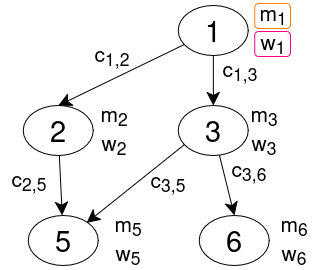
\includegraphics[scale=0.4]{diagrams/images/weights-noparts-rand.png}      
        \end{figure}
        }}
        \only<2>{   
        \raggedleft{
         \begin{figure}
            \centering
            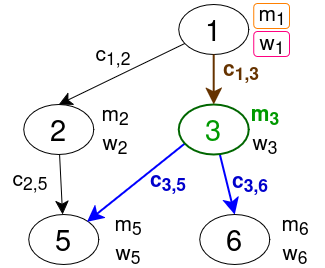
\includegraphics[scale=0.4]{diagrams/images/CCGRID-workflow-weights-for-ru.png}      
        \end{figure}
        }}
     
        
    \end{columns}   

    ~~~~~~~~~~~

 \only<2>{
\begin{figure}
                \centering
                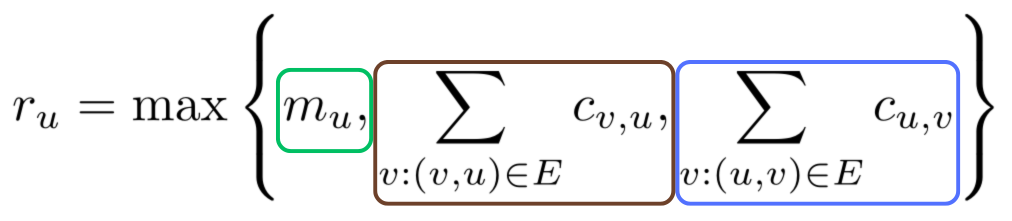
\includegraphics[width=0.5\linewidth]{diagrams/images/ru_formula_ccgrid_colors.png}                
                \label{fig:enter-label}
      \end{figure}

      }

\end{frame}


%%%%%%%%%%%%%%%%%%%%%%%%%%%%%%%%%%%%%%%%%%%%%%%%%%%
\begin{frame}[t]
    \frametitle{Model: Execution Environment}
   

    ~~~~~
    
    
 

      \begin{columns}
      \column{0.05\textwidth}
        \column{0.4\textwidth}
         \begin{itemize}
             \item Each processor has 

             \begin{itemize}
                 \item a limited memory of size $M_j$ and a communication buffer $MC_j$
                 \item speed $s_j$
             \end{itemize}

             \uncover<3,4>{
             \item Keep track of ready times on each
                  \begin{itemize}
                      \item Communication channel: $rt_{j,j'}$
                      \item Communication buffer:  $rt_j$
                  \end{itemize}  
                  }
         \end{itemize}
       
        \column{0.4\textwidth}
        \raggedleft{
         \begin{figure}
            \centering
            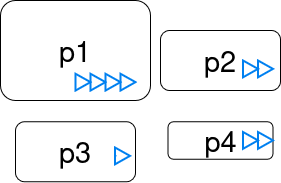
\includegraphics[scale=0.35]{diagrams/images/ClusterCCGRID.png}
            
            %\caption{Caption }
        \end{figure}

        \uncover<2,3,4>{
            \begin{figure}
            \centering
            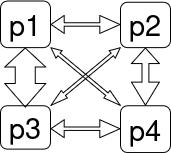
\includegraphics[scale=0.4]{diagrams/images/clusterCommunications.png}
            
            %\caption{Caption }
        \end{figure}
        }
        }
        \column{0.1\textwidth}
    \end{columns}   

    ~~~~~~~~~~~

\uncover<4>{
   Objective: makespan minimization with memory constraints
   }


\end{frame}


%%%%%%%%%%%%%%%%%%%%%%%%%%%%%%%%%%%%%%%%%%%%%%%%%%%
\begin{frame}[t]
    \frametitle{HEFT (in our model)}


  \begin{columns}
     \column{0.05\textwidth}
        \column{0.65\textwidth}
  HEFT~[1]:

  \begin{itemize}
      \item Assign each task a rank 
      \item Schedule tasks in decreasing rank order
     \only<2>{ \begin{itemize}
          \item Tentatively assign the task to each processor
          \item Choose the one with shortest finish time
      \end{itemize}
      }
  \end{itemize}
  
 \column{0.34\textwidth}
  \begin{tikzpicture}
   % \draw (4,2) ellipse (2cm and 1cm) node {What about memory?};
  \end{tikzpicture}

       % \column{0.1\textwidth}
    \end{columns}   

\uncover<2>{ 
  \begin{figure}
      \centering
        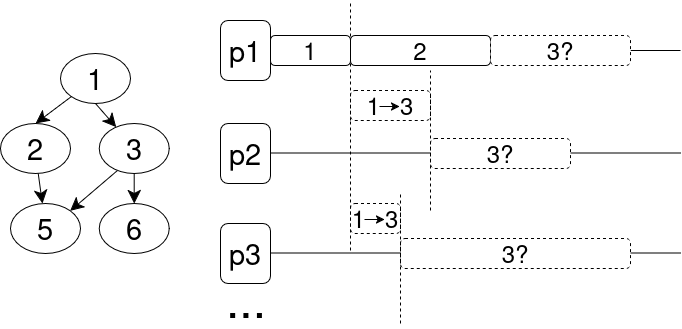
\includegraphics[scale=0.33]{diagrams/images/HEFT.png}
         %\caption{Caption }
  \end{figure}
  \vspace{-0.4cm}
  }



\footnotesize{[1] H. Topcuoglu, S. Hariri, M.-Y. Wu. Performance-effective and
low-complexity task scheduling for heterogeneous computing. 2002.}
 
\end{frame}


%%%%%%%%%%%%%%%%%%%%%%%%%%%%%%%%%%%%%%%%%%%%%%%%%%%
\begin{frame}[t]
    \frametitle{HEFT (in our model)}


  \begin{columns}

    \column{0.05\textwidth}
        \column{0.65\textwidth}
  HEFT~[1]:

  \begin{itemize}
      \item Assign each task a rank 
      \item Schedule tasks in decreasing rank order
      \begin{itemize}
          \item Tentatively assign the task to each processor
          \item Choose the one with shortest finish time
      \end{itemize}
  \end{itemize}
  
 \column{0.34\textwidth}
  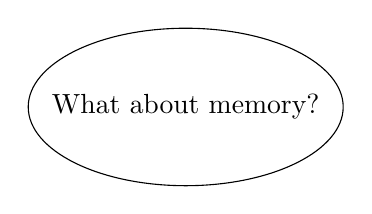
\begin{tikzpicture}
    \draw (4,2) ellipse (2cm and 1cm) node {What about memory?};
  \end{tikzpicture}

       % \column{0.1\textwidth}
    \end{columns}   

  \begin{figure}
      \centering
        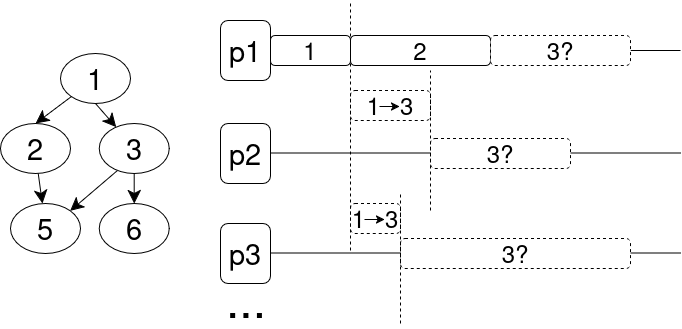
\includegraphics[scale=0.33]{diagrams/images/HEFT.png}
         %\caption{Caption }
  \end{figure}

\vspace{-0.4cm}
\footnotesize{[1] H. Topcuoglu, S. Hariri, M.-Y. Wu. Performance-effective and
low-complexity task scheduling for heterogeneous computing. 2002.}


 
\end{frame}

%%%%%%%%%%%%%%%%%%%%%%%%%%%%%%%%%%%%%%%%%%%%%%%%%%%
\begin{frame}[t]
    \frametitle{Memory Traversal}

    Fit into limited memory $\rightarrow$ use as little memory as possible

    ~~~~~~~~~~~~~~

  Peak memory depends on the traversal 

    
 \begin{columns}
      \column{0.05\textwidth}
        \column{0.6\textwidth}
     \begin{itemize}            
               \item Traversal $1 \rightarrow 3 \rightarrow 2$ 
             \begin{itemize}
                \item Execution of 3: $\textcolor{blue}{1000} (c_{1,2})+ \textcolor{blue}{10} (m_3) = 1011$
                \item Execution of 2: $\textcolor{blue}{1000} (m_2) + \textcolor{blue}{1} (c_{1,2}) = 1001$
            \end{itemize}
            \item Traversal $1 \rightarrow 2 \rightarrow 3$ 
            \begin{itemize}
                \item Execution of 2: $\textcolor{blue}{1000} (m_2)+ \textcolor{blue}{1} (c_{1,2}) + \textcolor{blue}{1000} (c_{1,3}) = 2001$
            \end{itemize}         

            \item Memory-optimal traversal \textsc{MemDag} [1]
                       
        \end{itemize}

      \column{0.3\textwidth}
        \raggedleft{
        %\vspace{-2.0cm}
         \begin{figure}
            \centering
            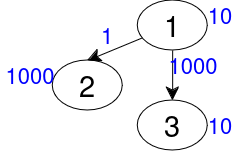
\includegraphics[scale=0.4]{diagrams/images/MemTraversal.png}
            %\caption{Caption }
        \end{figure}
        }
        \column{0.05\textwidth}
    \end{columns}  

%\vfill
~~~~~~~~~~~~~

 \footnotesize {[1] Kayaaslan, E., Lambert, T., Marchal, L., U{\c{c}}ar, B. (2018). Scheduling series-parallel task graphs to minimize peak memory. Theoretical Computer Science, 707, 1-23.}

 ~~~~~~
\end{frame}


%%%%%%%%%%%%%%%%%%%%%%%%%%%%%%%%%%%%%%%%%%%%%%%%%%%
\begin{frame}[t]
    \frametitle{Scenario and Model: Eviction}
   

      When a task executes, it
        
         \begin{itemize}
             \item consumes (deletes from memory) its incoming files,
             \item creates (inserts into memory) its outgoing files.

             \end{itemize}              
   
  To fit a task into memory, we may need to evict pending memories into the communication buffer
      

          \begin{figure}
            \centering
            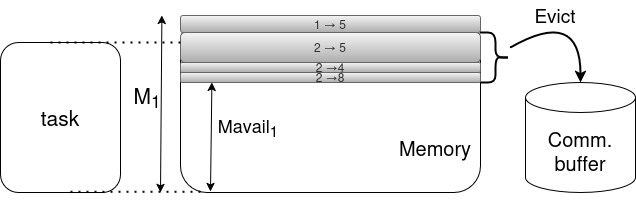
\includegraphics[scale=0.4]{diagrams/images/evictionCCGRID.png}    
        \end{figure}
       
No returning tasks back into memory!


\end{frame}




%%%%%%%%%%%%%%%%%%%%%%%%%%%%%%%%%%%%%%%%%%%%%
\begin{frame}[t]
    \frametitle{HEFTM-* heuristics: Ranking}
    
    Similar 2 phases to HEFT: rank and assign. \\[0.5ex]
    Implementation of the phases different.

 ~~~~~
\pause

  ~~~~~

   
    \begin{itemize}
        \item HEFTM-\textbf{BL}: orders by non-increasing bottom levels
        \item HEFTM-\textbf{BLC}: same, but prioritizes tasks with large incoming communications \\ 
            \begin{figure}
            \centering
            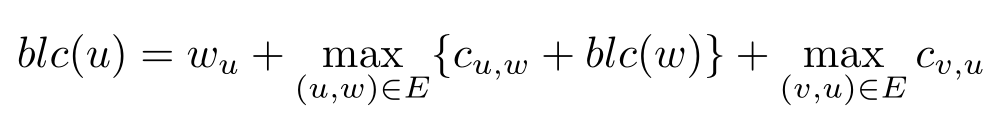
\includegraphics[scale=0.2]{diagrams/images/BLC-formula.png}
            %\caption{Caption }
        \end{figure}
        
        \item HEFTM-\textbf{MM}: orders according to \textsc{MemDag}'s memory-optimal traversal
        
    \end{itemize}
     
 
   

\end{frame}

%%%%%%%%%%%%%%%%%%%%%%%%%%%%%%%%%%%%%%%%%%%%%
\begin{frame}[t]
    \frametitle{HEFTM-* heuristics: Task Assignment}
    ~~~~~
    
 For each task $v$, \textbf{tentatively} try it on each processor $p_j$

  \begin{itemize}
      \item Check that for all predecessors assigned to $p_j$ the data is still in memory $\rightarrow$ otherwise invalid choice
      \item Address the memory constraint on the processor \\

       \begin{figure}
            \centering
            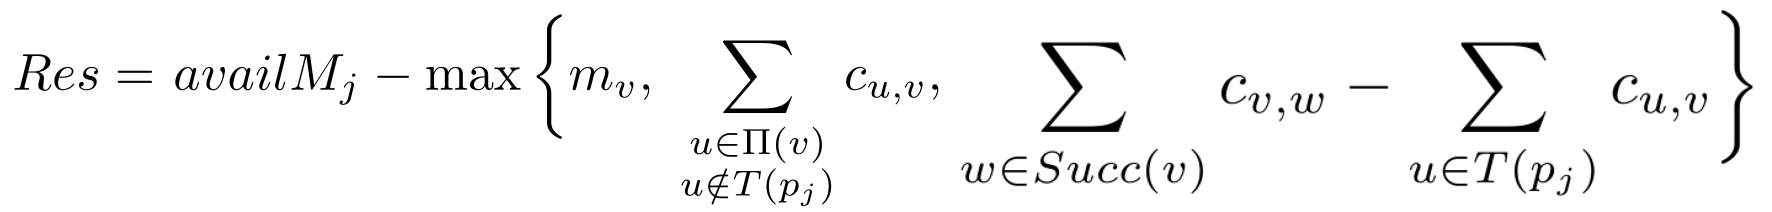
\includegraphics[width=.7\textwidth]{diagrams/images/Res-formula}
        \end{figure}
  \end{itemize}

    \begin{center}
        \uncover<2>{
            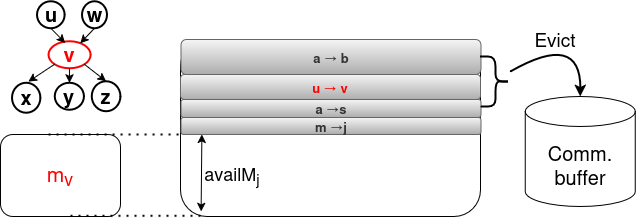
\includegraphics[scale=0.4]{diagrams/images/CCgridEvict1}
        }
    \end{center}


\end{frame}

%%%%%%%%%%%%%%%%%%%%%%%%%%%%%%%%%%%%%%%%%%%%%
\begin{frame}[t]
    \frametitle{HEFTM-* heuristics: Task Assignment}
    ~~~~~

    Greedily assign each task $v$ to processor $p_j$ that minimizes finish time.

    \begin{itemize}
        \item Check that for all predecessors assigned to $p_j$ the data is still in memory $\rightarrow$ otherwise invalid choice
        \item Address the memory constraint on the processor \\

        \begin{figure}
            \centering
            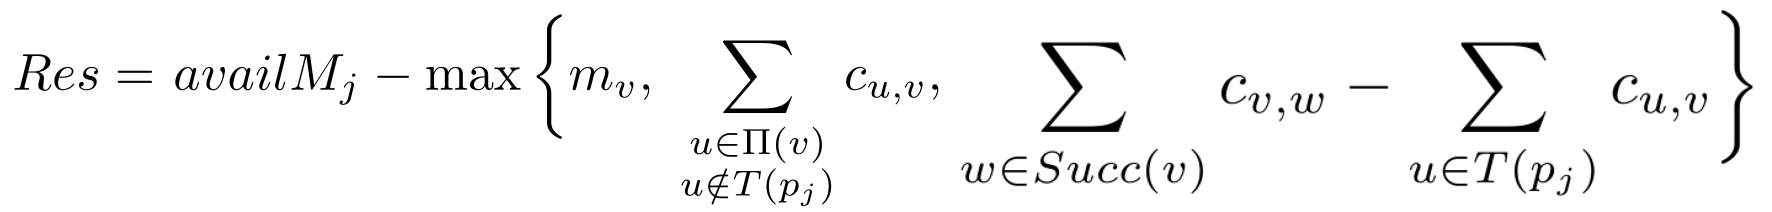
\includegraphics[width=.7\textwidth]{diagrams/images/Res-formula}
        \end{figure}
    \end{itemize}

    \begin{center}
            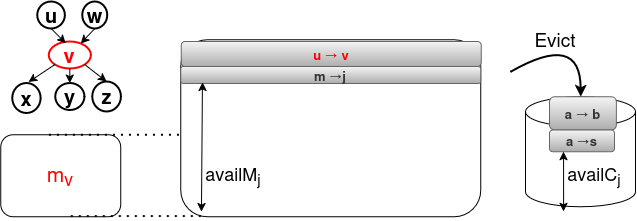
\includegraphics[scale=0.4]{diagrams/images/CCgridEvict2}
    \end{center}

\end{frame}
%%%%%%%%%%%%%%%%%%%%%%%%%%%%%%%%%%%%%%%%%%%%%

\begin{frame}[t]
    \frametitle{Start and Finish Time Calculation}

    % --- Put background image using TikZ ---
    \begin{tikzpicture}[remember picture, overlay]
        \node[anchor=south east, xshift=0cm, yshift=1.5cm] at (current page.south east) {
            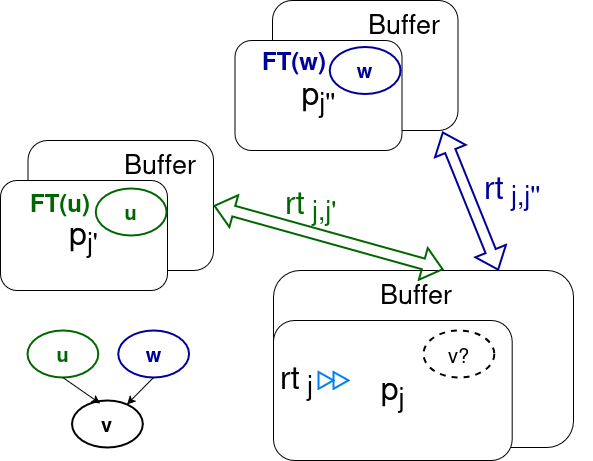
\includegraphics[width=0.55\paperwidth]{diagrams/images/StartTime.png}
        };
    \end{tikzpicture}

     \vspace{-0.6cm}
       % --- Foreground content (text appears over image) ---
    \begin{itemize}
        \item Start after all communications have finished
        \begin{figure}
            \centering
            \hskip -5.5cm
            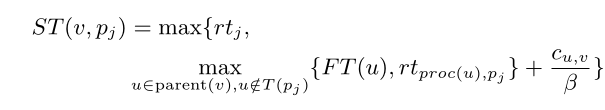
\includegraphics[width=.6\textwidth]{diagrams/images/formula-starttime-paperwithrts.png}
        \end{figure}

    \end{itemize}

    \begin{columns}
        \column{0.02\textwidth}
        \column{0.35\textwidth}
        \begin{itemize}
            \item  Finish time
            \begin{align*}
                FT(v, p_j) &= \\
                &ST(v, p_j) + \frac{w_v}{s_j}
            \end{align*}
        \end{itemize}
        \column{0.6\textwidth}
        \column{0.08\textwidth}
    \end{columns}


    \begin{overlayarea}{\paperwidth}{\paperheight}
            \begin{tikzpicture}[remember picture, overlay]
                \draw[red, thick]
                ([xshift=-9.8cm,yshift=7.5cm]current page.south east)
                ellipse (0.5cm and 0.5cm);
            \end{tikzpicture}
    \end{overlayarea}

\end{frame}
%%%%%%%%%%%%%%%%%%%%%%%%%%%%%%%%%%%%%%%%%%%%%
%%%%%%%%%%%%%%%%%%%%%%%%%%%%%%%%%%%%%%%%%%%%

\begin{frame}[t]
    \frametitle{Start and Finish Time Calculation}

    % --- Put background image using TikZ ---
    \begin{tikzpicture}[remember picture, overlay]
        \node[anchor=south east, xshift=0cm, yshift=1.5cm] at (current page.south east) {
            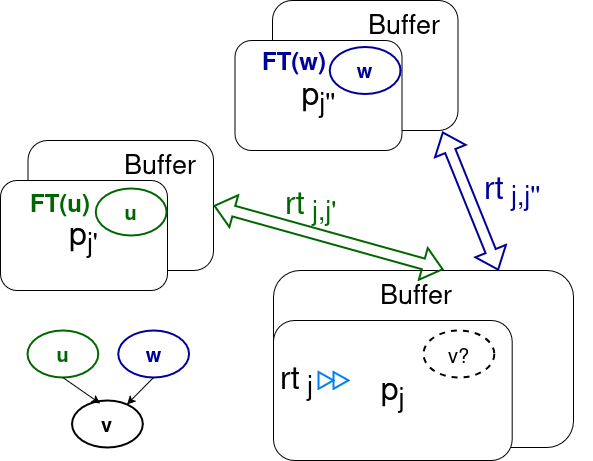
\includegraphics[width=0.55\paperwidth]{diagrams/images/StartTime.png}
        };
    \end{tikzpicture}

    \vspace{-0.6cm}
    % --- Foreground content (text appears over image) ---
    \begin{itemize}
        \item Start after all communications have finished
        \begin{figure}
            \centering
            \hskip -5.5cm
            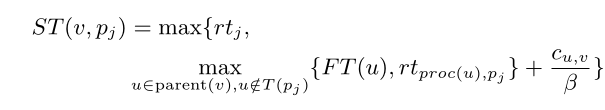
\includegraphics[width=.6\textwidth]{diagrams/images/formula-starttime-paperwithrts.png}
        \end{figure}

    \end{itemize}

    \begin{columns}
        \column{0.02\textwidth}
        \column{0.35\textwidth}
        \begin{itemize}
            \item  Finish time
            \begin{align*}
                FT(v, p_j) &= \\
                &ST(v, p_j) + \frac{w_v}{s_j}
            \end{align*}
        \end{itemize}
        \column{0.6\textwidth}
        \column{0.08\textwidth}
    \end{columns}


    \begin{overlayarea}{\paperwidth}{\paperheight}
        \begin{tikzpicture}[remember picture, overlay]
            \draw[red, thick]
            ([xshift=-8.4cm,yshift=6.8cm]current page.south east)
            ellipse (0.5cm and 0.5cm);
        \end{tikzpicture}
    \end{overlayarea}

\end{frame}

%%%%%%%%%%%%%%%%%%%%%%%%%%%%%%%%%%%%%%%%%%%%

\begin{frame}[t]
    \frametitle{Start and Finish Time Calculation}

    % --- Put background image using TikZ ---
    \begin{tikzpicture}[remember picture, overlay]
        \node[anchor=south east, xshift=0cm, yshift=1.5cm] at (current page.south east) {
            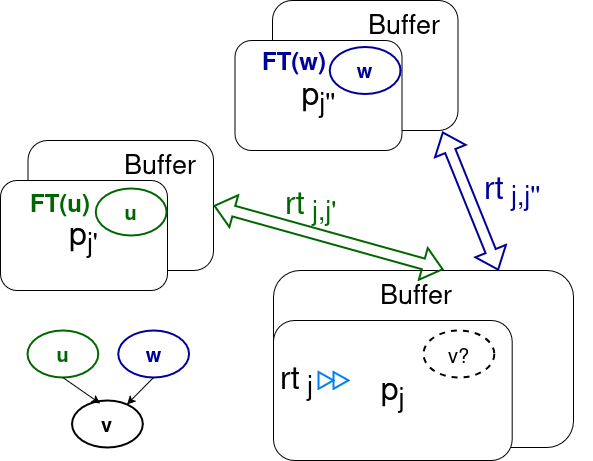
\includegraphics[width=0.55\paperwidth]{diagrams/images/StartTime.png}
        };
    \end{tikzpicture}

    \vspace{-0.6cm}
    % --- Foreground content (text appears over image) ---
    \begin{itemize}
        \item Start after all communications have finished
        \begin{figure}
            \centering
            \hskip -5.5cm
            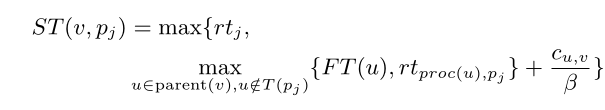
\includegraphics[width=.6\textwidth]{diagrams/images/formula-starttime-paperwithrts.png}
        \end{figure}

    \end{itemize}

    \begin{columns}
        \column{0.02\textwidth}
        \column{0.35\textwidth}
        \begin{itemize}
            \item  Finish time
            \begin{align*}
                FT(v, p_j) &= \\
                &ST(v, p_j) + \frac{w_v}{s_j}
            \end{align*}
        \end{itemize}
        \column{0.6\textwidth}
        \column{0.08\textwidth}
    \end{columns}


    \begin{overlayarea}{\paperwidth}{\paperheight}
        \begin{tikzpicture}[remember picture, overlay]
            \draw[red, thick]
            ([xshift=-7.0cm,yshift=6.8cm]current page.south east)
            ellipse (1.0cm and 0.5cm);
        \end{tikzpicture}
    \end{overlayarea}

\end{frame}
%%%%%%%%%%%%%%%%%%%%%%%%%%%%%%%%%%%%%%%%%%%%%%%%%%%

\begin{frame}[t]
    \frametitle{Final Assignment}


    Final assignment to processor

    \begin{itemize}
        \item Evict files that need to be evicted from memory,
        \begin{itemize}
            \item  remove them from pending memory and add to communication buffer
            \item reduce buffers sizes accordingly
        \end{itemize}
        \item New $availM_j$: - eviction, - incoming files, + outgoing files
        \item For each predecessor on another processor $j'$: ready time on communication buffer $rt_{j, j'}$

    \end{itemize}

\end{frame}

%%%%%%%%%%%%%%%%%%%%%%%%%%%%%%%%%%%%%%%%%%%%%



\begin{frame}[t]
    \frametitle{Experimental Setup}

    ~~~~~~~~~~~~~~~~~~~~~~~

    Schedule real (scientific) workflows \\[0.35ex]
    
    Task and edge weights: historical data from Lotaru [6]

    ~~~~~~~~~~~~~~~~~~~

        \begin{itemize}  
        \item Workflows
        \begin{itemize}
             \item Real-world workflows
            \item Generated with WFGen [7] from 7 workflow: sizes from 1K to 30K tasks
            \item Divided in groups by size
        \end{itemize}          
     
        \item Execution environments
         \begin{itemize}
             \item 36 processors: 6 pieces of same 6 kinds of processors as in [6]
            \item Memory-constrained: same processors, 10 times less memory
        \end{itemize} 
    \end{itemize}    

~~~~~~~~~~~~~~~~~~~~~~~~


\footnotesize{[6] Bader, J., Lehmann, F., Thamsen, L., Will, J., Leser, U., and Kao, O. 2022. Lotaru: Locally Estimating Runtimes of Scientific Workflow Tasks in Heterogeneous Clusters. SSDBM.}

\footnotesize{[7] Coleman, T., Casanova, H., Pottier, L., Kaushik, M., Deelman, E., and da Silva, R. F. 2022. WfCommons: A framework for enabling scientific
workflow research and development. Future Generation Computer Systems.}

\end{frame}
%%%%%%%%%%%%%%%%%%%%%%%%%%%%%%%%%%%%%%%%%%%%%

\begin{frame}[t]
    \frametitle{Results}
    \framesubtitle{Default cluster - Success Rates}
   
    \vspace{-0.8cm}
    \begin{figure}    
        \centering
         \hskip -0.5cm
        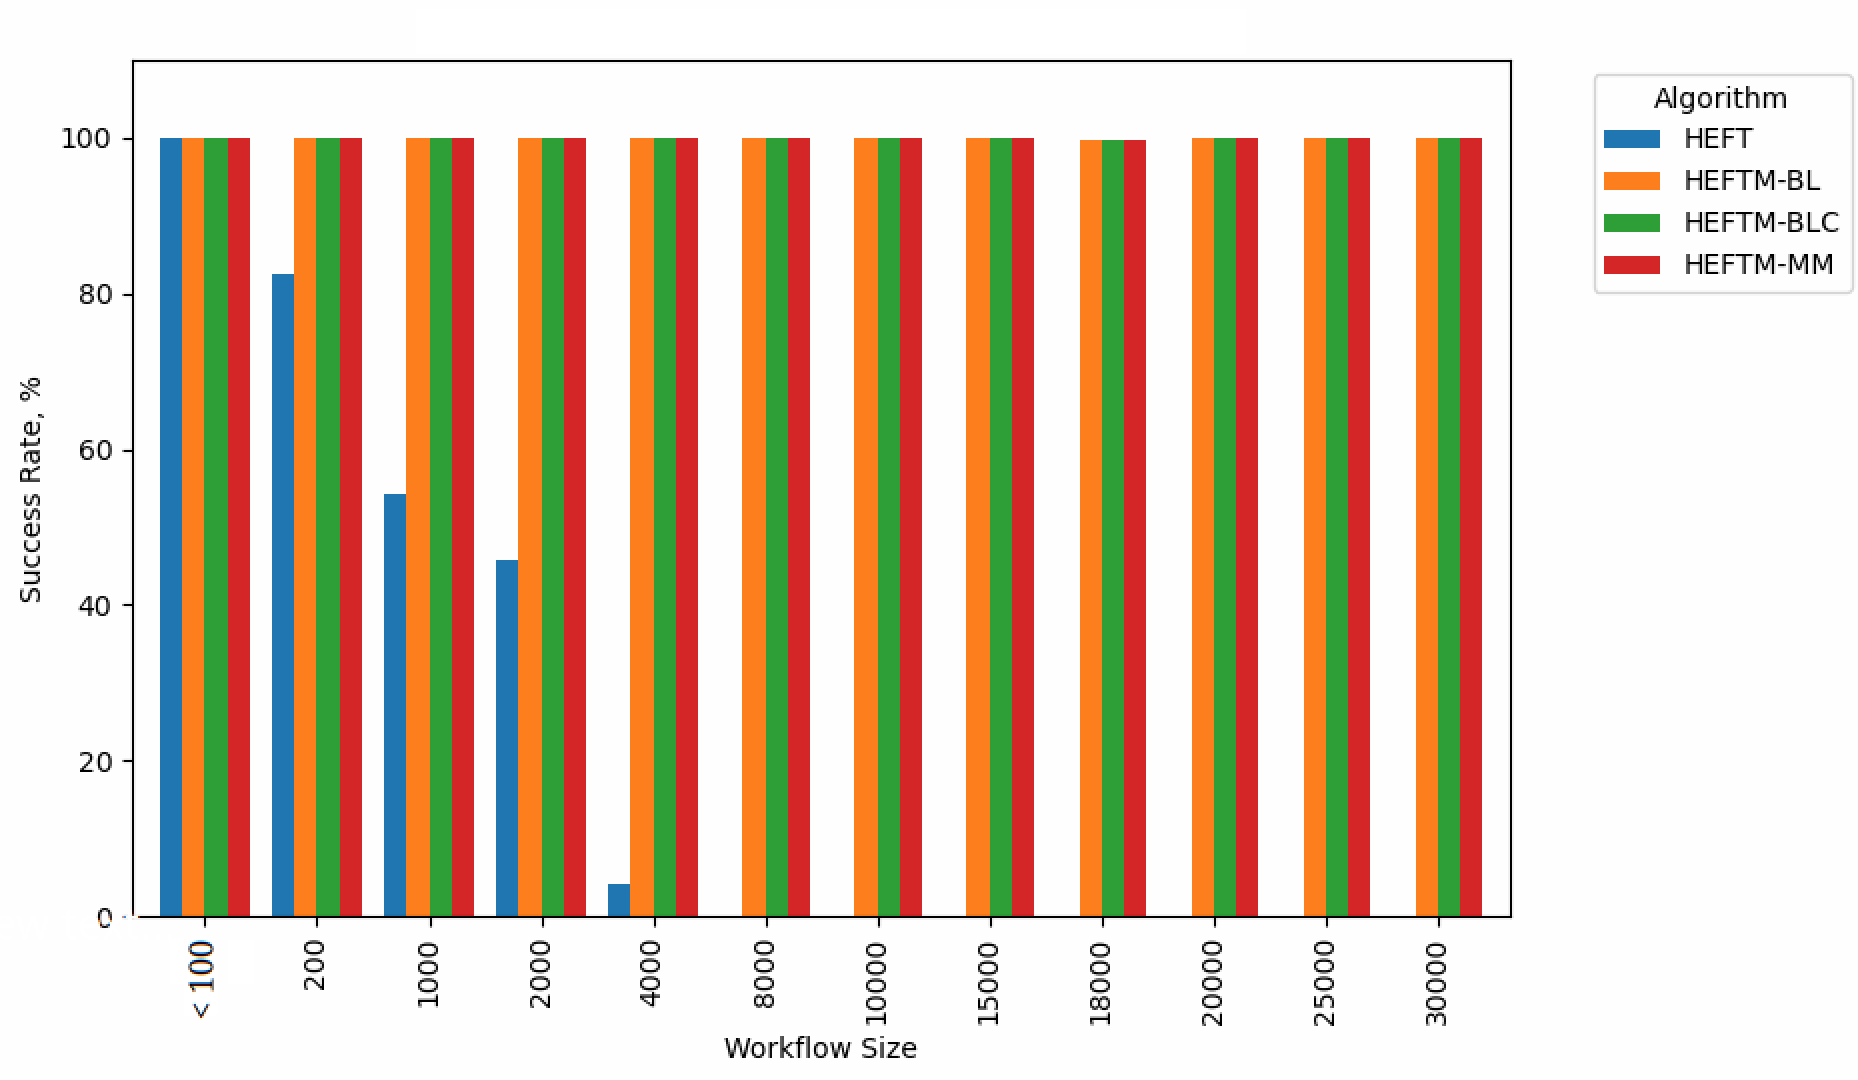
\includegraphics[scale=0.38]{diagrams/images/success-rates-large2.png}
        % \caption{Makespans of HomPart in comparison to HetPart1.}
    \end{figure}

    % Overlay rectangle on top
    \begin{tikzpicture}[remember picture, overlay]
        \node[
            fill=white,
            draw=black,
            rounded corners,
            minimum width=4cm,
            minimum height=1.5cm,
            align=center
        ] at ([xshift=-5cm,yshift=-4.5cm]current page.north east)
        {HEFT invalid over 2000 tasks \\ \\ HEFTM-* valid for all workflows };
    \end{tikzpicture}

\end{frame}


%%%%%%%%%%%%%%%%%%%%%%%%%%%%%%%%%%%%%%%%%%%%%

\begin{frame}[t]
    \frametitle{Results}
    \framesubtitle{Default cluster - Relative Makespans}

      \begin{textblock*}{5cm}(7cm,4cm) % {block width} (coords)
        %HEFT fails, HEFTM-* valid
    \end{textblock*}
    
     \vspace{-0.2cm}
        \begin{figure}
            \centering
            \hskip -0.7cm
            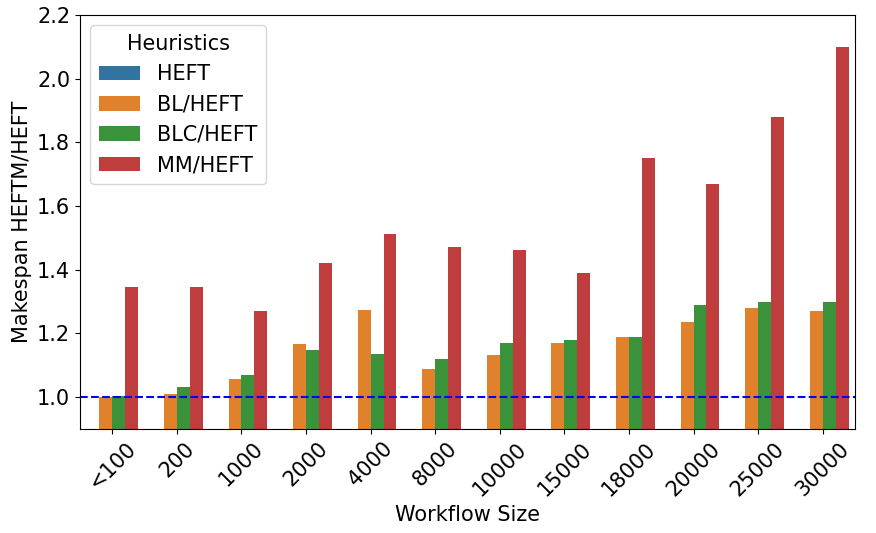
\includegraphics[scale=0.36]{diagrams/images/ms_relations_by_wf_size_barplot.png}
          %  \caption{Runtimes of HetPart2 in comparison to HetPart 1. }
        \end{figure}

    \begin{tikzpicture}[remember picture, overlay]
            \node[
                fill=white,
                draw=black,
                rounded corners,
                minimum width=4cm,
                minimum height=1.5cm,
                align=center
            ] at ([xshift=-5cm,yshift=-3.8cm]current page.north east)
            {HEFTM-* makespans valid, HEFT not \\ HEFTM-BL and BLC : 10 - 35\% worse \\ HEFTM-MM makespans 40\% to 2x worse};
        \end{tikzpicture}


\end{frame}


%%%%%%%%%%%%%%%%%%%%%%%%%%%%%%%%%%%%%%%%%%%%%

\begin{frame}[t]
    \frametitle{Results}
    \framesubtitle{Memory-Constrained Cluster: Success Rates}

      \vspace{-0.3cm}
        \begin{figure}
            \centering
            \hskip -0.5cm
            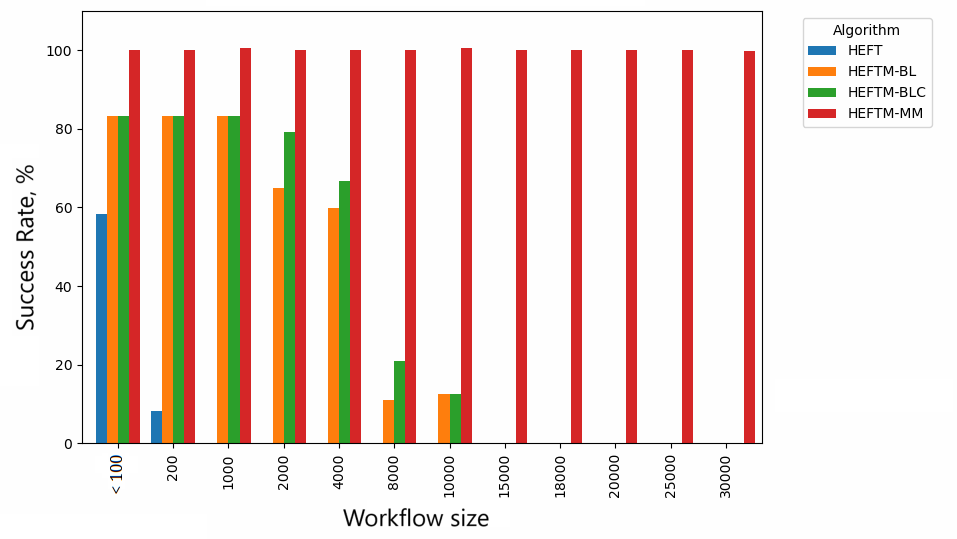
\includegraphics[scale=1.25]{diagrams/images/success-rates-tiny.png}
           % \caption{Makespans of HomPart in comparison to HetPart1.}
        \end{figure} 


          \begin{tikzpicture}[remember picture, overlay]
        \node[
            fill=white,
            draw=black,
            rounded corners,
            minimum width=4cm,
            minimum height=1.5cm,
            align=center
        ] at ([xshift=-3.5cm,yshift=-5.5cm]current page.north east)
        {HEFT invalid over 100 tasks \\ HEFTM-BL / HEFTM-BLC invalid over  \\8000 tasks
        \\ HEFTM-* valid for all workflows };
    \end{tikzpicture}

    \begin{tikzpicture}[remember picture, overlay]
        \node[
            fill=white,
            draw=black,
            rounded corners,
            minimum width=3.0cm,
            minimum height=1.5cm,
            align=center
        ] at ([xshift=-3.7cm,yshift=-1.8cm]current page.north east)
            {\textcolor{red}{\parbox{2.9cm}{Less realistic, \\extreme strain for\\ the algorithm}}};
    \end{tikzpicture}

   \end{frame}

   
%%%%%%%%%%%%%%%%%%%%%%%%%%%%%%%%%%%%%%%%%%%%%

\begin{frame}[t]
    \frametitle{Results}
    \framesubtitle{Memory-Constrained Cluster: Relative Makespans}
         \vspace{-0.8cm}
        \begin{figure}
            \centering
            \hskip -0.8cm
            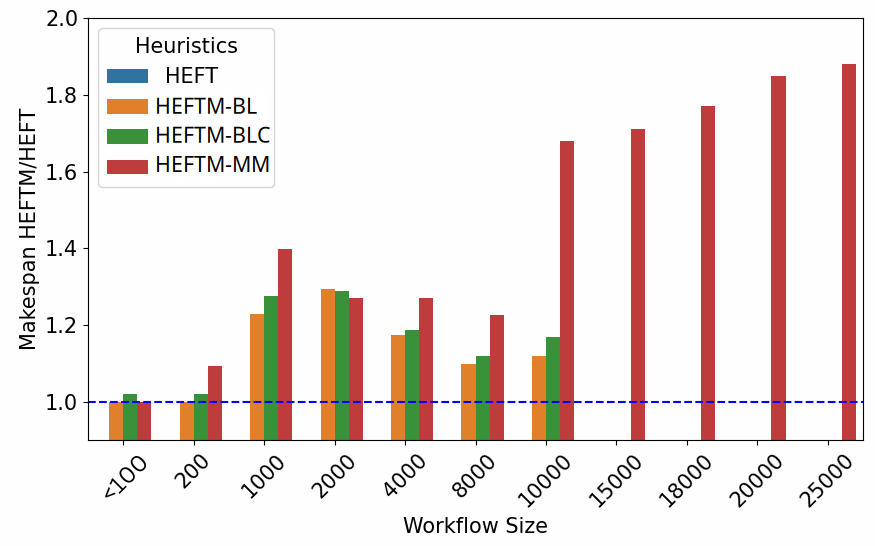
\includegraphics[scale=0.48]{diagrams/images/ms_relations_by_wf_size-constrained-barplot.png}
          %  \caption{Runtimes of HetPart2 in comparison to HetPart 1. }
        \end{figure}

        
    \begin{tikzpicture}[remember picture, overlay]
        \node[
            fill=white,
            draw=black,
            rounded corners,
            minimum width=4cm,
            minimum height=1.5cm,
            align=center
        ] at ([xshift=-5.0cm,yshift=-4.5cm]current page.north east)
        {Most makespans invalid, \\
        even by HEFTM-BL and HEFTM-BLC; \\ HEFTM-MM makespans the only valid ones };
    \end{tikzpicture}
   \end{frame}

%%%%%%%%%%%%%%%%%%%%%%%%%%%%%%%%%%%%%%%%%%%%%

\begin{frame}[t]
    \frametitle{Results}
    \framesubtitle{Runtime}

    \makebox[0pt][l]{\hspace{-1.0cm}%
        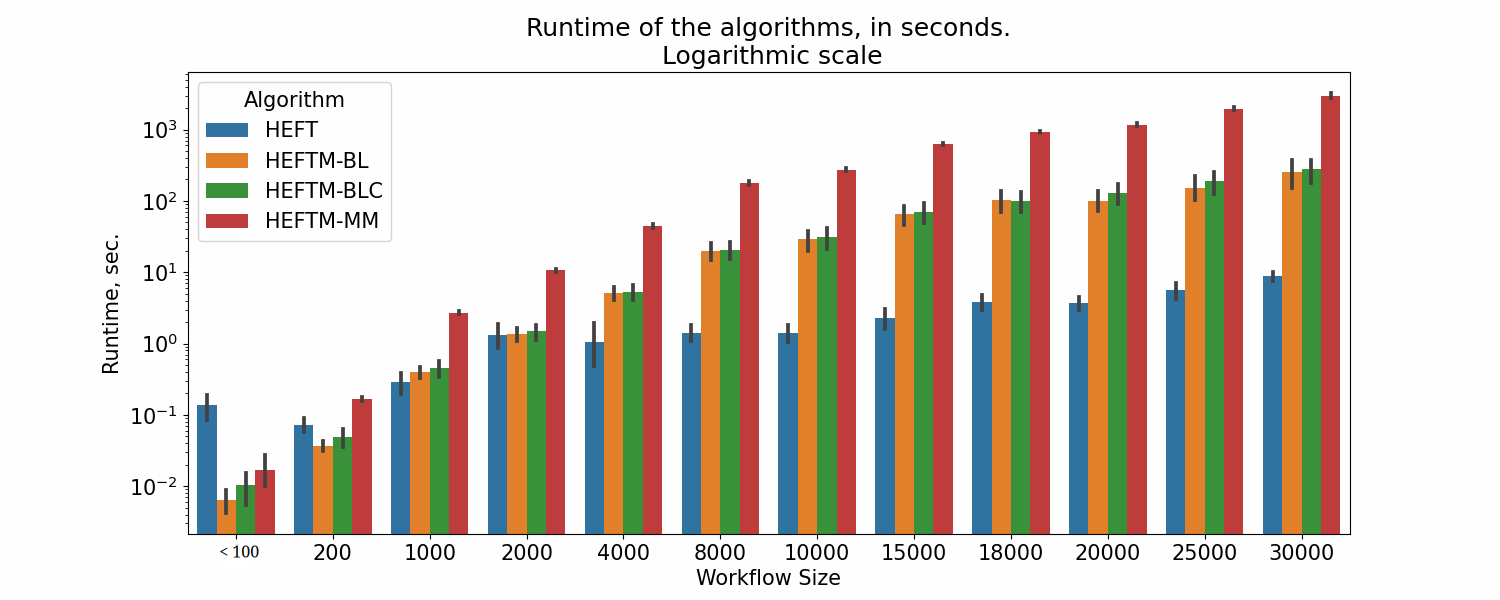
\includegraphics[scale=0.26]{diagrams/images/runtimes-logarithmic.png}
    }

    \begin{tikzpicture}[remember picture, overlay]
        \node[
            fill=white,
            draw=black,
            rounded corners,
            minimum width=4.8cm,
            minimum height=1.7cm,
            align=center
        ] at ([xshift=-4.5cm,yshift=-4.5cm]current page.north east)
        {Runtimes from 1/100 of seconds to minutes\\
         HEFTM-MM has longest runtimes\\
         Computation of optimal traversal costly};
    \end{tikzpicture}

\end{frame}

%%%%%%%%%%%%%%%%%%%%%%%%%%%%%%%%%%%%%%%%%%%%%

\begin{frame}
\frametitle{Adaptive scenario}
\vspace{-2.0cm}

\begin{itemize}
    \item No perfect knowledge of task runtimes and memory usage
    \item Workflow changes: more/less memory, more/less time to execute
\end{itemize}

\vspace{-0.5cm}
 \uncover<2>{ 
 \begin{columns}

    %\column{0.05\textwidth}
    \column{0.69\textwidth}
     \begin{figure}    
        \centering
         %\hskip -0.5cm
        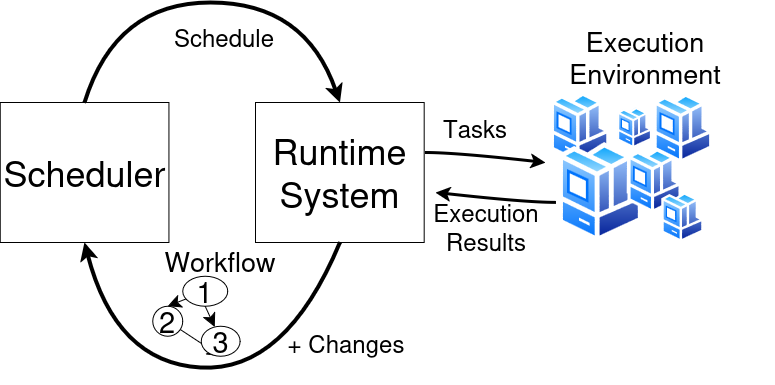
\includegraphics[scale=0.3]{diagrams/images/schedulerAndRUntime.png}
        % \caption{Makespans of HomPart in comparison to HetPart1.}
    \end{figure}
    \column{0.29\textwidth}
   Runtime reports changes

       \begin{itemize}
        \item Can invalidate - not enough memory anymore
        \item Can lead to later finish time
     
    \end{itemize}

\end{columns}

 }


\end{frame}


%%%%%%%%%%%%%%%%%%%%%%%%%%%%%%%%%%%%%%%%%%%%%

\begin{frame}
    \frametitle{Adaptive Scenario}

    No recomputation: the majority of schedules becomes invalid!
   
      
        \begin{figure}
            \centering
            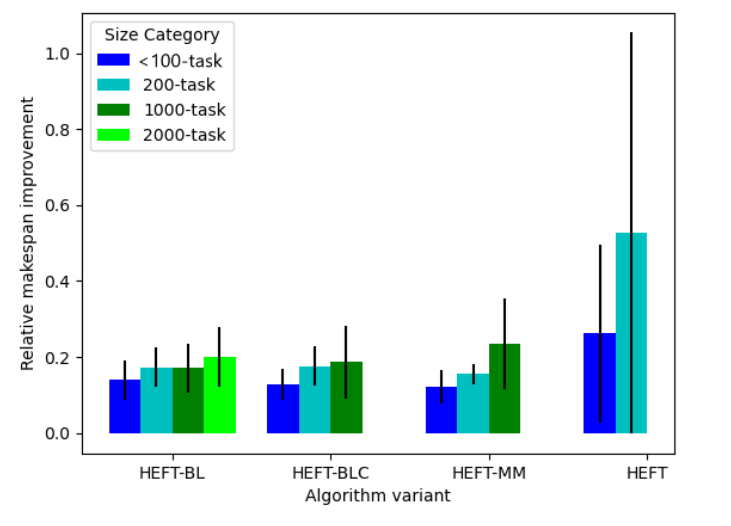
\includegraphics[scale=0.3]{diagrams/images/MsImprovDynamicCCGRID.png}
          
        \end{figure}
   
\end{frame}


%%%%%%%%%%%%%%%%%%%%%%%%%%%%%%%%%%%%%%%%%%%%%
\begin{frame}[t]
    \frametitle{Summary}
\framesubtitle{HEFTM-*: memory-valid schedules for each taste!}

\begin{itemize}
    \item Extend an influential predecessor (HEFT)
    \item Memory-aware, communicate over communication buffers
    \item Valid makespans, only 10-35\% worse than invalid HEFT makespans
    \item HEFT-\textbf{MM} proves unique resilience in memory-constrained scenario
\end{itemize}

\pause
    \begin{table}[ht]
        \centering
        \setlength{\tabcolsep}{12pt} % adjust horizontal padding between columns
        \renewcommand{\arraystretch}{1.3} % increase row height for readability
        \begin{tabular}{|p{6.5cm}|p{2.5cm}|}
            \hline
            \textbf{Scenario} & \textbf{Winner} \\
            \hline
            Memory very constrained & HEFT-\textbf{MM} \\
            Memory somewhat constrained, need smallest makespan & HEFTM-\textbf{BL} \\
            Need balance, willing to trade (very little) makespan for less memory requirement & HEFTM-\textbf{BLC} \\
            Lots of memory, need smallest makespan & \only<1>{HEFT?} \only<2> {\sout{HEFT} ~~~~~~~ HEFTM-\textbf{BL}} \\
            \hline
        \end{tabular}
    \end{table}


\end{frame}


%%%%%%%%%%%%%%%%%%%%%%%%%%%%%%%%%%%%%%%%%%%%%%%%%%%%%%%%
\begin{frame}
    \centering
    \Large{Thank you!}
    
    \vspace{2cm}
    
    \small{This work is partially supported by Collaborative Research Center (CRC) 1404 FONDA – Foundations of Workflows for Large-Scale Scientific Data
Analysis, which is funded by German Research Foundation (DFG).}

\end{frame}




%%%%%%%%%%%%%%%%%%%%%%%%%%%%%%%%%%%%%%%%%%%%%
\begin{frame}% [t]
    \frametitle{Future Work}

TBD


\end{frame}


%%%%%%%%%%%%%%%%%%%%%%%%%%%%%%%%%%%%%%%%%%%%%%%%%%%%%%%%%%
\begin{frame}[t]
    \frametitle{Previous Work}

TBD 
     \begin{columns}
     %\column{0.05\textwidth}
        \column{0.4\textwidth}
        \begin{itemize}
            \item Tree-shaped, then DAG-shaped workflows
            \item Makespan minimization, memory-aware
            \item Mapping only, no adaptive scenarios
        \end{itemize}
        \column{0.4\textwidth}
        \begin{figure}
        \vspace{-1cm}
            \centering
           % \includegraphics[scale=0.15]{diagrams/partitions.png}
            %\caption{Caption }
        \end{figure}
         \column{0.05\textwidth}
    \end{columns}

    ~~~~~~~~~~~~~

    ~~~~~~~~~~~~~~~~~~~~
     
    \begin{tabular}{|c||c||c|c|}
        \hline
        & Gou et al.~[2] & HetPart1~[3] & HetPart2~[4]  \\
        \hline
        Memory & \cellcolor{pink}homogeneous & \cellcolor{lime} heterogeneous & \cellcolor{lime}heterogeneous\\
        \hline
        Processor speeds & \cellcolor{pink}homogeneous & \cellcolor{pink}homogeneous & \cellcolor{lime}heterogeneous\\
        \hline
    \end{tabular}
   % 
   % \vspace{\fill}

   ~~~~~~~~~~~~~~~~~~~~~~

~~~~~~~~~~~~~~~~~~~~~~~~~~~~

~~~~~~~~~~~~~~~~~~~~
    
    \footnotesize{[2] Gou, C., Benoit, A., Marchal, L.: Partitioning tree-shaped task graphs for distributed platforms with limited memory. IEEE Trans on Par and DistSystems 31(7), (2020)}
    
    \footnotesize{[3] Kulagina, S., Meyerhenke, H., Benoit, A.: Mapping Tree-shaped Workflows on Memory-heterogeneous Architectures. HeteroPar 2022} 
    
    \footnotesize{[4] Kulagina, S., Meyerhenke, H., Benoit, A.: Mapping Tree-shaped Workflows on Systems with Different Memory Sizes and Processor Speeds. Wiley's Concurrency and Computation Practice and Experience}

\end{frame}


\end{document}
